
\documentclass[border=8pt, multi, tikz]{standalone} 
\usepackage{import}
\subimport{../layers/}{init}
\usetikzlibrary{positioning}
\usetikzlibrary{3d} %for including external image 

\def\ConvColor{rgb:yellow,5;red,2.5;white,5}
\def\ConvReluColor{rgb:yellow,5;red,5;white,5}
\def\PoolColor{rgb:red,1;black,0.3}
\def\UnpoolColor{rgb:blue,2;green,1;black,0.3}
\def\FcColor{rgb:blue,5;red,2.5;white,5}
\def\FcReluColor{rgb:blue,5;red,5;white,4}
\def\SoftmaxColor{rgb:magenta,5;black,7}   
\def\SumColor{rgb:blue,5;green,15}

\newcommand{\copymidarrow}{\tikz \draw[-Stealth,line width=0.8mm,draw={rgb:blue,4;red,1;green,1;black,3}] (-0.3,0) -- ++(0.3,0);}

\begin{document}
\begin{tikzpicture}
\tikzstyle{connection}=[ultra thick,every node/.style={sloped,allow upside down},draw=\edgecolor,opacity=0.7]
\tikzstyle{copyconnection}=[ultra thick,every node/.style={sloped,allow upside down},draw={rgb:blue,4;red,1;green,1;black,3},opacity=0.7]

\node[canvas is zy plane at x=0] (temp) at (-3,0,0) {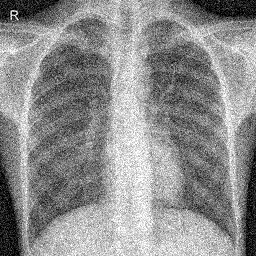
\includegraphics[width=8cm,height=8cm]{../examples/noisy.png}};

\pic[shift={(0,0,0)}] at (0,0,0) 
    {Box={
        name=ccr_b1a,
        caption= ,
        xlabel={{32, }},
        zlabel=256,
        fill=\ConvColor,
        height=40,
        width=2,
        depth=0
        }
    };

\pic[shift={(0.5, 0, 0)}] at (ccr_b1a-east) 
    {Box={
        name=ccr_b1,
        caption= ,
        xlabel={{32, }},
        zlabel=256,
        fill=\ConvColor,
        height=40,
        width=2,
        depth=0
        }
    };

\draw [connection]  (ccr_b1a-east)    -- node {\midarrow} (ccr_b1-west);

\pic[shift={ (0, -3, 0) }] at (ccr_b1-southwest) 
    {Box={
        name=pool_b2,
        caption= ,
        fill=\PoolColor,
        opacity=0.5,
        height=20,
        width=2,
        depth=0
        }
    };

\draw [connection]  (ccr_b1-southwest)    -- node {\midarrow} (pool_b2-northwest);

\pic[shift={(0.5, 0, 0)}] at (pool_b2-east) 
    {Box={
        name=ccr_b2a,
        caption= ,
        xlabel={{64, }},
        zlabel=128,
        fill=\ConvColor,
        height=20,
        width=4,
        depth=0
        }
    };

\pic[shift={(0.5, 0, 0)}] at (ccr_b2a-east) 
    {Box={
        name=ccr_b2,
        caption= ,
        xlabel={{64, }},
        zlabel=128,
        fill=\ConvColor,
        height=20,
        width=4,
        depth=0
        }
    };

\draw [connection]  (ccr_b2a-east)    -- node {\midarrow} (ccr_b2-west);

\draw [connection]  (pool_b2-east)    -- node {\midarrow} (ccr_b2a-west);

\pic[shift={ (0, -3, 0) }] at (ccr_b2-southwest) 
    {Box={
        name=pool_b3,
        caption= ,
        fill=\PoolColor,
        opacity=0.5,
        height=10,
        width=4,
        depth=0
        }
    };

\draw [connection]  (ccr_b2-southwest)    -- node {\midarrow} (pool_b3-northwest);

\pic[shift={(0.5, 0, 0)}] at (pool_b3-east) 
    {Box={
        name=ccr_b3a,
        caption= ,
        xlabel={{128, }},
        zlabel=64,
        fill=\ConvColor,
        height=10,
        width=8,
        depth=0
        }
    };

\pic[shift={(0.5, 0, 0)}] at (ccr_b3a-east) 
    {Box={
        name=ccr_b3,
        caption= ,
        xlabel={{128, }},
        zlabel=64,
        fill=\ConvColor,
        height=10,
        width=8,
        depth=0
        }
    };

\draw [connection]  (ccr_b3a-east)    -- node {\midarrow} (ccr_b3-west);

\draw [connection]  (pool_b3-east)    -- node {\midarrow} (ccr_b3a-west);

\pic[shift={ (0, -2, 0) }] at (ccr_b3-southwest) 
    {Box={
        name=pool_b4,
        caption= ,
        fill=\PoolColor,
        opacity=0.5,
        height=5,
        width=8,
        depth=0
        }
    };

\draw [connection]  (ccr_b3-southwest)    -- node {\midarrow} (pool_b4-northwest);

\pic[shift={(0.5, 0, 0)}] at (pool_b4-east) 
    {Box={
        name=ccr_b4a,
        caption= ,
        xlabel={{256, }},
        zlabel=32,
        fill=\ConvColor,
        height=5,
        width=16,
        depth=0
        }
    };

\pic[shift={(0.5, 0, 0)}] at (ccr_b4a-east) 
    {Box={
        name=ccr_b4,
        caption= ,
        xlabel={{256, }},
        zlabel=32,
        fill=\ConvColor,
        height=5,
        width=16,
        depth=0
        }
    };

\draw [connection]  (ccr_b4a-east)    -- node {\midarrow} (ccr_b4-west);

\draw [connection]  (pool_b4-east)    -- node {\midarrow} (ccr_b4a-west);

\pic[shift={ (0, 2.5, 0) }] at (ccr_b4-northwest) 
    {Box={
        name=unpool_b7,
        caption= ,
        fill=\UnpoolColor,
        opacity=0.5,
        height=10,
        width=8,
        depth=0
        }
    };

\pic[shift={(0, 0, 0)}] at (unpool_b7-east) 
    {Box={
        name=ccr_res_b7,
        caption= ,
        xlabel={{128, }},
        zlabel=64,
        fill=\ConvColor,
        height=10,
        width=8,
        depth=0
        }
    };

\draw [connection]  (ccr_b3-east)    -- node {\midarrow} (unpool_b7-west);

\draw [connection]  (ccr_b4-northeast)    -- node {\midarrow} (ccr_res_b7-southeast);

\pic[shift={(0.5, 0, 0)}] at (ccr_res_b7-east) 
    {Box={
        name=ccr_b7a,
        caption= ,
        xlabel={{128, }},
        zlabel=64,
        fill=\ConvColor,
        height=10,
        width=8,
        depth=0
        }
    };

\pic[shift={(0.5, 0, 0)}] at (ccr_b7a-east) 
    {Box={
        name=ccr_b7,
        caption= ,
        xlabel={{128, }},
        zlabel=64,
        fill=\ConvColor,
        height=10,
        width=8,
        depth=0
        }
    };

\draw [connection]  (ccr_b7a-east)    -- node {\midarrow} (ccr_b7-west);

\draw [connection]  (ccr_res_b7-east)    -- node {\midarrow} (ccr_b7a-west);

\pic[shift={ (0, 4, 0) }] at (ccr_b7-northwest) 
    {Box={
        name=unpool_b8,
        caption= ,
        fill=\UnpoolColor,
        opacity=0.5,
        height=20,
        width=4,
        depth=0
        }
    };

\pic[shift={(0, 0, 0)}] at (unpool_b8-east) 
    {Box={
        name=ccr_res_b8,
        caption= ,
        xlabel={{64, }},
        zlabel=128,
        fill=\ConvColor,
        height=20,
        width=4,
        depth=0
        }
    };

\draw [connection]  (ccr_b2-east)    -- node {\midarrow} (unpool_b8-west);

\draw [connection]  (ccr_b7-northeast)    -- node {\midarrow} (ccr_res_b8-southeast);

\pic[shift={(0.5, 0, 0)}] at (ccr_res_b8-east) 
    {Box={
        name=ccr_b8a,
        caption= ,
        xlabel={{64, }},
        zlabel=128,
        fill=\ConvColor,
        height=20,
        width=4,
        depth=0
        }
    };

\pic[shift={(0.5, 0, 0)}] at (ccr_b8a-east) 
    {Box={
        name=ccr_b8,
        caption= ,
        xlabel={{64, }},
        zlabel=128,
        fill=\ConvColor,
        height=20,
        width=4,
        depth=0
        }
    };

\draw [connection]  (ccr_b8a-east)    -- node {\midarrow} (ccr_b8-west);

\draw [connection]  (ccr_res_b8-east)    -- node {\midarrow} (ccr_b8a-west);

\pic[shift={ (0, 5, 0) }] at (ccr_b8-northwest) 
    {Box={
        name=unpool_b9,
        caption= ,
        fill=\UnpoolColor,
        opacity=0.5,
        height=40,
        width=2,
        depth=0
        }
    };

\pic[shift={(0, 0, 0)}] at (unpool_b9-east) 
    {Box={
        name=ccr_res_b9,
        caption= ,
        xlabel={{32, }},
        zlabel=256,
        fill=\ConvColor,
        height=40,
        width=2,
        depth=0
        }
    };

\draw [connection]  (ccr_b1-east)    -- node {\midarrow} (unpool_b9-west);

\draw [connection]  (ccr_b8-northeast)    -- node {\midarrow} (ccr_res_b9-southeast);

\pic[shift={(0.5, 0, 0)}] at (ccr_res_b9-east) 
    {Box={
        name=ccr_b9a,
        caption= ,
        xlabel={{32, }},
        zlabel=256,
        fill=\ConvColor,
        height=40,
        width=2,
        depth=0
        }
    };

\pic[shift={(0.5, 0, 0)}] at (ccr_b9a-east) 
    {Box={
        name=ccr_b9,
        caption= ,
        xlabel={{32, }},
        zlabel=256,
        fill=\ConvColor,
        height=40,
        width=2,
        depth=0
        }
    };

\draw [connection]  (ccr_b9a-east)    -- node {\midarrow} (ccr_b9-west);

\draw [connection]  (ccr_res_b9-east)    -- node {\midarrow} (ccr_b9a-west);

\pic[shift={(0.75, 0, 0)}] at (ccr_b9-east) 
    {Box={
        name=soft1,
        caption= ,
        zlabel=256,
        fill=\SoftmaxColor,
        height=40,
        width=0.5,
        depth=0
        }
    };

\draw [connection]  (ccr_b9-east)    -- node {\midarrow} (soft1-west);

\end{tikzpicture}
\end{document}
